%
% einleitung.tex -- Beispiel-File für die Einleitung
%
% (c) 2020 Prof Dr Andreas Müller, Hochschule Rapperswil
%
% !TEX root = ../../buch.tex
% !TEX encoding = UTF-8
%
\subsection{Zylinder\label{geodaeten:section:Linienelemente:Zylinder}}
\rhead{Linienelemente Beispiele}

Eine Kurve auf der Oberfläche eines Zylinders kann als zweidimensional betrachtet werden, wobei gilt
\begin{equation}
	\Delta s \approx \sqrt{(r \cdot \Delta \phi)^2 + \Delta z^2}
\end{equation}
wenn $r$ konstant ist.
Analog zu den kartesischen Koordinaten können die Abstände infinitesimal werden und das Linienelement für die Oberfläche des Zylinders ergibt sich dadurch zu
\begin{equation}
	ds^2 = r^2 \cdot d \phi^2 + d z^2 .
	\label{geodaeten:equation:Linienelemente:Zylinder:equation2}
\end{equation}

Den Einstieg in dreidimensionale Kurven können wir machen, indem $r$ als nicht konstant angenommen wird.
Der Weg kann so mit
\begin{equation}
	\Delta s \approx \sqrt{\Delta r^2 + (r \cdot \Delta \phi)^2 + \Delta z^2} %\cdot dt^2
\end{equation}
berechnet werden und das Linienelement entspricht 
\begin{equation}
	ds^2 = d r^2 + r^2 \cdot d \phi^2 + d z^2 .
	\label{geodaeten:equation:Linienelemente:Zylinder:Zylinder3D}
\end{equation}

\begin{figure}
	\centering
	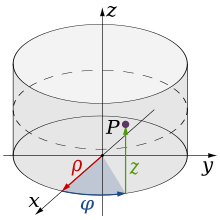
\includegraphics[width=4cm]{papers/geodaeten/Abbildungen/Linienelemente/LinZyl1}
	\caption{zylindrischer Raum mit $r = \rho$. Bildquelle: \cite{geodaeten:polarkoordinaten}}
	\label{geodaeten:figure:Linienelemente:Zylinder:figure2}
	
\end{figure}